\documentclass[12pt]{article}
%\documentclass[a6paper]{article}
\usepackage{amsmath}
\usepackage{amssymb}
\usepackage{amsthm}
\usepackage{graphicx}
\usepackage{rotating}
\usepackage{lscape}
\usepackage{enumerate}
\usepackage{booktabs}
\usepackage{subfig}
\usepackage{changepage}
\usepackage{geometry}
%\usepackage{natbib}
\usepackage{xcolor}
\usepackage{setspace}
\usepackage{hyperref}
%\usepackage{breqn}
\usepackage{float}
\usepackage{xcolor,colortbl} 
\geometry{letterpaper, portrait, margin=1in}

\usepackage{graphicx}
\graphicspath{ {./graphs/} }

\title{CLT optimization}
\author{Maxwell Spivakovsky}

\begin{document}
\maketitle
\section{CLT}
In \cite{CLT} an algorithm for aligning two cell lineage trees is proposed. The algorithm is based on dynamic programming, choosing an alignment that optimizes the score between two trees. There are two external inputs to the algorithm: (1) the score matrix between the cell type of any terminal node of tree A and the cell type of any terminal node of tree B and (2) the pruning cost of leaving out a tree node of either tree A or tree B from the aligned tree. As mentioned in the \cite{CLT} both of these are crucial to the results of alignment. Yet there is no theoretical model that selects these parameters; in the examples in the paper the scores used are either 2 or 0 and the pruning cost is chosen to be 1. There is a section that describes a greedy algorithm for choosing each score from a small number of available scores, but the algorithm relies on the assumption of the pruning cost that is fixed at 10, 20, 40, and 80 at each of the four rounds of the algorithm. \\
The main difficulty in relating the score matrix and the pruning cost to the output alignment score is that the dynamic programming algorithm is recursive by nature. To align two trees, each on the order of a thousand nodes requires the order of a million evaluations, where each evaluation may depend on the results of four other evaluations. This recursion makes the dependence on the score matrix and the pruning cost highly non-linear. But each evaluation on its own is a continuous function of the parameters, more specifically, the maximum of the results of several continuous evaluations, where the maximum corresponds to the dynamic programming nature of the solution. Deep learning packages like pyTorch are well suited for both recursive evaluations and for optimizing a piecewise linear objective function. The approach taken below treats the alignment score as a function of the score matrix and the tuning cost parameter and optimizes an objective function of these parameters. This not only optimizes the score matrix and the tuning cost separately but also accounts for how these parameters influence each other. The objective function that is optimized is not simply the alignment score between the two trees, the score matrix that produces a high alignment score could be aligning completely unrelated cells. Instead, the objective function maximizes the alignment score between two trees relative to the alignment scores of the random trees, constructed by randomly permuting the terminal nodes of each tree while keeping the rest of the structure unchanged. Let the alignment score between two trees, A and B be denoted as
\begin{equation*}
  A(a,b)
\end{equation*}
Let \(a_{\sigma^a}\) denote a tree that has the same structure as tree \(a\) but whose terminal nodes have been permuted according to the permutation \(\sigma^a\). Suppose \(N\) such permutations are carried out and their mean and standard deviation are computed:
\begin{gather*}
  \mu = {\frac 1 N} \sum_{i=1}^N A(a_{\sigma^a_i},b_{\sigma^b_i}) \\
  \sigma^2 = {\frac 1 N} \sum_{i=1}^N  \Bigl( A(a_{\sigma^a_i},b_{\sigma^b_i}) - \mu \Bigr)^2 \\
\end{gather*}
These quantities depend on the score matrix \(S\) and pruning cost \(p\). The objective function is
\begin{equation*}
  F(S,p) = {\frac { A(a,b)-\mu} \sigma}
\end{equation*}
Maximizing \(F(S,p)\) is choosing \(S,p\) that results in the highest alignment score of the two trees relative to the alignment scores of randomly permuted trees. The intention is that \(S,p\) are capturing the relationship between the two trees, both the geometry of each tree separately, as well as the geometry of their combination. Optimization is done with pyTorch in the typical deep learning fashion: a batch of random trees is created and \(F(S,p)\) is evaluated with respect to that batch. pyTorch computes the gradient of \(F(S,p)\) and modifies the values of \(S\) and \(p\). Then another batch is created, different from the preceding one, and the process is repeated. It takes around 10,000 batches to converge to a solution. The matrix \(S\) is normalized to the unit norm at each step by applying \(softmax\) to \(S\). Below is a typical convergence profile of the model:

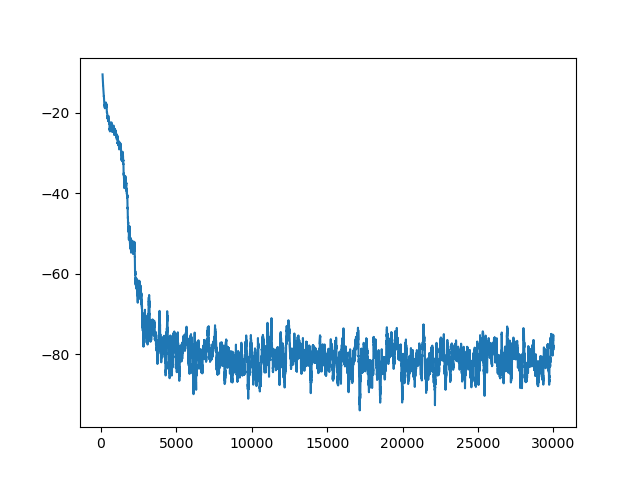
\includegraphics[width=\textwidth]{ave_loss.png}

the x-axis is the number of batches. the y-axis shows by how many standard deviations the average batch's permuted trees alignment score is lower than the alignment score of the actual trees. This quantity is calculated on each batch before the score matrix and the pruning cost is changed after processing the batch so that the random trees in that batch have not been incorporated into optimization.\\
\subsection{Optimal score matrix for a tree}
When a tree is aligned with itself perfect alignment is expected. Intuitively, optimization should place high scores on matching a cell type from tree 1 to the same cell type of tree 2. There are 3 lineage trees in the GitHub that corresponds to the results in \cite{CLT}. The names of the three trees are 'fun','pma', and 'hro'. 'fun' seems to correspond to {\it Caenorhabditis elegans}, 'pma' to {\it P. marina}. For each of the three trees, the optimizer selected the optimal score matrix when aligning the tree to itself. Since tree 1 and tree 2 correspond to the same organism the score matrix was constrained to be symmetric. The results are below.

\begin{table}[H]
\begin{center}
\resizebox{\linewidth}{!}{%
\begin{tabular}{lrrrrrrrrr}
\toprule
 & BLA & DEA & EPI & GER & GLA & INT & MUS & NEU & STR \\
\midrule
BLA & {\cellcolor[HTML]{90D083}} \color[HTML]{000000} \bfseries 0.069614 & {\cellcolor[HTML]{FCFED6}} \color[HTML]{000000} 0.007390 & {\cellcolor[HTML]{FFFFE5}} \color[HTML]{000000} 0.000220 & {\cellcolor[HTML]{FEFFE1}} \color[HTML]{000000} 0.002148 & {\cellcolor[HTML]{FEFFDF}} \color[HTML]{000000} 0.002704 & {\cellcolor[HTML]{FCFED4}} \color[HTML]{000000} 0.007579 & {\cellcolor[HTML]{FFFFE5}} \color[HTML]{000000} 0.000349 & {\cellcolor[HTML]{FFFFE4}} \color[HTML]{000000} 0.000673 & {\cellcolor[HTML]{FFFFE5}} \color[HTML]{000000} 0.000080 \\
DEA & {\cellcolor[HTML]{FCFED6}} \color[HTML]{000000} 0.007390 & {\cellcolor[HTML]{C5E89A}} \color[HTML]{000000} \bfseries 0.048439 & {\cellcolor[HTML]{FFFFE5}} \color[HTML]{000000} 0.000558 & {\cellcolor[HTML]{F3FAB6}} \color[HTML]{000000} 0.022470 & {\cellcolor[HTML]{FFFFE4}} \color[HTML]{000000} 0.000884 & {\cellcolor[HTML]{FAFDCB}} \color[HTML]{000000} 0.012193 & {\cellcolor[HTML]{FFFFE5}} \color[HTML]{000000} 0.000153 & {\cellcolor[HTML]{FEFFE2}} \color[HTML]{000000} 0.001751 & {\cellcolor[HTML]{FFFFE5}} \color[HTML]{000000} 0.000141 \\
EPI & {\cellcolor[HTML]{FFFFE5}} \color[HTML]{000000} 0.000220 & {\cellcolor[HTML]{FFFFE5}} \color[HTML]{000000} 0.000558 & {\cellcolor[HTML]{C1E698}} \color[HTML]{000000} \bfseries 0.050339 & {\cellcolor[HTML]{FDFED9}} \color[HTML]{000000} 0.005938 & {\cellcolor[HTML]{FEFFE2}} \color[HTML]{000000} 0.001458 & {\cellcolor[HTML]{FFFFE5}} \color[HTML]{000000} 0.000376 & {\cellcolor[HTML]{FFFFE4}} \color[HTML]{000000} 0.000750 & {\cellcolor[HTML]{FFFFE5}} \color[HTML]{000000} 0.000016 & {\cellcolor[HTML]{FEFFDE}} \color[HTML]{000000} 0.003547 \\
GER & {\cellcolor[HTML]{FEFFE1}} \color[HTML]{000000} 0.002148 & {\cellcolor[HTML]{F3FAB6}} \color[HTML]{000000} 0.022470 & {\cellcolor[HTML]{FDFED9}} \color[HTML]{000000} 0.005938 & {\cellcolor[HTML]{004529}} \color[HTML]{F1F1F1} \bfseries 0.157615 & {\cellcolor[HTML]{FFFFE5}} \color[HTML]{000000} 0.000364 & {\cellcolor[HTML]{FFFFE5}} \color[HTML]{000000} 0.000605 & {\cellcolor[HTML]{F8FCC0}} \color[HTML]{000000} 0.016638 & {\cellcolor[HTML]{FCFED6}} \color[HTML]{000000} 0.007050 & {\cellcolor[HTML]{F9FDC2}} \color[HTML]{000000} 0.015871 \\
GLA & {\cellcolor[HTML]{FEFFDF}} \color[HTML]{000000} 0.002704 & {\cellcolor[HTML]{FFFFE4}} \color[HTML]{000000} 0.000884 & {\cellcolor[HTML]{FEFFE2}} \color[HTML]{000000} 0.001458 & {\cellcolor[HTML]{FFFFE5}} \color[HTML]{000000} 0.000364 & {\cellcolor[HTML]{5AB76A}} \color[HTML]{F1F1F1} \bfseries 0.089513 & {\cellcolor[HTML]{FDFEDB}} \color[HTML]{000000} 0.004575 & {\cellcolor[HTML]{FAFDC8}} \color[HTML]{000000} 0.012991 & {\cellcolor[HTML]{FBFED2}} \color[HTML]{000000} 0.008902 & {\cellcolor[HTML]{EDF8B1}} \color[HTML]{000000} 0.026936 \\
INT & {\cellcolor[HTML]{FCFED4}} \color[HTML]{000000} 0.007579 & {\cellcolor[HTML]{FAFDCB}} \color[HTML]{000000} 0.012193 & {\cellcolor[HTML]{FFFFE5}} \color[HTML]{000000} 0.000376 & {\cellcolor[HTML]{FFFFE5}} \color[HTML]{000000} 0.000605 & {\cellcolor[HTML]{FDFEDB}} \color[HTML]{000000} 0.004575 & {\cellcolor[HTML]{77C679}} \color[HTML]{000000} \bfseries 0.078844 & {\cellcolor[HTML]{FFFFE5}} \color[HTML]{000000} 0.000169 & {\cellcolor[HTML]{FFFFE4}} \color[HTML]{000000} 0.000941 & {\cellcolor[HTML]{FEFFE2}} \color[HTML]{000000} 0.001295 \\
MUS & {\cellcolor[HTML]{FFFFE5}} \color[HTML]{000000} 0.000349 & {\cellcolor[HTML]{FFFFE5}} \color[HTML]{000000} 0.000153 & {\cellcolor[HTML]{FFFFE4}} \color[HTML]{000000} 0.000750 & {\cellcolor[HTML]{F8FCC0}} \color[HTML]{000000} 0.016638 & {\cellcolor[HTML]{FAFDC8}} \color[HTML]{000000} 0.012991 & {\cellcolor[HTML]{FFFFE5}} \color[HTML]{000000} 0.000169 & {\cellcolor[HTML]{CEEB9E}} \color[HTML]{000000} \bfseries 0.044478 & {\cellcolor[HTML]{FFFFE5}} \color[HTML]{000000} 0.000404 & {\cellcolor[HTML]{FCFED7}} \color[HTML]{000000} 0.006591 \\
NEU & {\cellcolor[HTML]{FFFFE4}} \color[HTML]{000000} 0.000673 & {\cellcolor[HTML]{FEFFE2}} \color[HTML]{000000} 0.001751 & {\cellcolor[HTML]{FFFFE5}} \color[HTML]{000000} 0.000016 & {\cellcolor[HTML]{FCFED6}} \color[HTML]{000000} 0.007050 & {\cellcolor[HTML]{FBFED2}} \color[HTML]{000000} 0.008902 & {\cellcolor[HTML]{FFFFE4}} \color[HTML]{000000} 0.000941 & {\cellcolor[HTML]{FFFFE5}} \color[HTML]{000000} 0.000404 & {\cellcolor[HTML]{DDF1A6}} \color[HTML]{000000} \bfseries 0.037532 & {\cellcolor[HTML]{FDFEDD}} \color[HTML]{000000} 0.004220 \\
STR & {\cellcolor[HTML]{FFFFE5}} \color[HTML]{000000} 0.000080 & {\cellcolor[HTML]{FFFFE5}} \color[HTML]{000000} 0.000141 & {\cellcolor[HTML]{FEFFDE}} \color[HTML]{000000} 0.003547 & {\cellcolor[HTML]{F9FDC2}} \color[HTML]{000000} 0.015871 & {\cellcolor[HTML]{EDF8B1}} \color[HTML]{000000} 0.026936 & {\cellcolor[HTML]{FEFFE2}} \color[HTML]{000000} 0.001295 & {\cellcolor[HTML]{FCFED7}} \color[HTML]{000000} 0.006591 & {\cellcolor[HTML]{FDFEDD}} \color[HTML]{000000} 0.004220 & {\cellcolor[HTML]{9CD687}} \color[HTML]{000000} \bfseries 0.065764 \\
\bottomrule
\end{tabular}
}\end{center}
\caption{fun aligned with fun}\end{table}
\begin{table}[H]
\begin{center}
\resizebox{\linewidth}{!}{%
\begin{tabular}{lrrrrrrrr}
\toprule
 & ? & EPI & GER & INT & MUS & NER & PHA & X \\
\midrule
? & {\cellcolor[HTML]{7AC77A}} \color[HTML]{000000} \bfseries 0.107569 & {\cellcolor[HTML]{FFFFE5}} \color[HTML]{000000} 0.000359 & {\cellcolor[HTML]{F3FAB6}} \color[HTML]{000000} 0.030688 & {\cellcolor[HTML]{FAFDC9}} \color[HTML]{000000} 0.017442 & {\cellcolor[HTML]{FFFFE5}} \color[HTML]{000000} 0.000731 & {\cellcolor[HTML]{FFFFE5}} \color[HTML]{000000} 0.000040 & {\cellcolor[HTML]{FEFFE2}} \color[HTML]{000000} 0.002285 & {\cellcolor[HTML]{FFFFE5}} \color[HTML]{000000} 0.000146 \\
EPI & {\cellcolor[HTML]{FFFFE5}} \color[HTML]{000000} 0.000359 & {\cellcolor[HTML]{CBEA9C}} \color[HTML]{000000} \bfseries 0.063155 & {\cellcolor[HTML]{FFFFE5}} \color[HTML]{000000} 0.000767 & {\cellcolor[HTML]{F8FDC1}} \color[HTML]{000000} 0.022299 & {\cellcolor[HTML]{FFFFE5}} \color[HTML]{000000} 0.000057 & {\cellcolor[HTML]{FFFFE5}} \color[HTML]{000000} 0.000278 & {\cellcolor[HTML]{FFFFE5}} \color[HTML]{000000} 0.000054 & {\cellcolor[HTML]{FDFEDD}} \color[HTML]{000000} 0.005833 \\
GER & {\cellcolor[HTML]{F3FAB6}} \color[HTML]{000000} 0.030688 & {\cellcolor[HTML]{FFFFE5}} \color[HTML]{000000} 0.000767 & {\cellcolor[HTML]{004529}} \color[HTML]{F1F1F1} \bfseries 0.216988 & {\cellcolor[HTML]{FFFFE4}} \color[HTML]{000000} 0.001329 & {\cellcolor[HTML]{FEFFE2}} \color[HTML]{000000} 0.002331 & {\cellcolor[HTML]{FFFFE4}} \color[HTML]{000000} 0.001100 & {\cellcolor[HTML]{FEFFE2}} \color[HTML]{000000} 0.002389 & {\cellcolor[HTML]{FFFFE4}} \color[HTML]{000000} 0.001176 \\
INT & {\cellcolor[HTML]{FAFDC9}} \color[HTML]{000000} 0.017442 & {\cellcolor[HTML]{F8FDC1}} \color[HTML]{000000} 0.022299 & {\cellcolor[HTML]{FFFFE4}} \color[HTML]{000000} 0.001329 & {\cellcolor[HTML]{55B567}} \color[HTML]{F1F1F1} \bfseries 0.125486 & {\cellcolor[HTML]{FFFFE4}} \color[HTML]{000000} 0.001374 & {\cellcolor[HTML]{FFFFE5}} \color[HTML]{000000} 0.000019 & {\cellcolor[HTML]{FEFFDF}} \color[HTML]{000000} 0.003746 & {\cellcolor[HTML]{FFFFE5}} \color[HTML]{000000} 0.000202 \\
MUS & {\cellcolor[HTML]{FFFFE5}} \color[HTML]{000000} 0.000731 & {\cellcolor[HTML]{FFFFE5}} \color[HTML]{000000} 0.000057 & {\cellcolor[HTML]{FEFFE2}} \color[HTML]{000000} 0.002331 & {\cellcolor[HTML]{FFFFE4}} \color[HTML]{000000} 0.001374 & {\cellcolor[HTML]{AFDE8F}} \color[HTML]{000000} \bfseries 0.080111 & {\cellcolor[HTML]{FFFFE5}} \color[HTML]{000000} 0.000002 & {\cellcolor[HTML]{FFFFE5}} \color[HTML]{000000} 0.000031 & {\cellcolor[HTML]{FFFFE5}} \color[HTML]{000000} 0.000006 \\
NER & {\cellcolor[HTML]{FFFFE5}} \color[HTML]{000000} 0.000040 & {\cellcolor[HTML]{FFFFE5}} \color[HTML]{000000} 0.000278 & {\cellcolor[HTML]{FFFFE4}} \color[HTML]{000000} 0.001100 & {\cellcolor[HTML]{FFFFE5}} \color[HTML]{000000} 0.000019 & {\cellcolor[HTML]{FFFFE5}} \color[HTML]{000000} 0.000002 & {\cellcolor[HTML]{CBEA9C}} \color[HTML]{000000} \bfseries 0.063512 & {\cellcolor[HTML]{FFFFE4}} \color[HTML]{000000} 0.001003 & {\cellcolor[HTML]{FFFFE5}} \color[HTML]{000000} 0.000761 \\
PHA & {\cellcolor[HTML]{FEFFE2}} \color[HTML]{000000} 0.002285 & {\cellcolor[HTML]{FFFFE5}} \color[HTML]{000000} 0.000054 & {\cellcolor[HTML]{FEFFE2}} \color[HTML]{000000} 0.002389 & {\cellcolor[HTML]{FEFFDF}} \color[HTML]{000000} 0.003746 & {\cellcolor[HTML]{FFFFE5}} \color[HTML]{000000} 0.000031 & {\cellcolor[HTML]{FFFFE4}} \color[HTML]{000000} 0.001003 & {\cellcolor[HTML]{C3E698}} \color[HTML]{000000} \bfseries 0.068355 & {\cellcolor[HTML]{FFFFE5}} \color[HTML]{000000} 0.000151 \\
X & {\cellcolor[HTML]{FFFFE5}} \color[HTML]{000000} 0.000146 & {\cellcolor[HTML]{FDFEDD}} \color[HTML]{000000} 0.005833 & {\cellcolor[HTML]{FFFFE4}} \color[HTML]{000000} 0.001176 & {\cellcolor[HTML]{FFFFE5}} \color[HTML]{000000} 0.000202 & {\cellcolor[HTML]{FFFFE5}} \color[HTML]{000000} 0.000006 & {\cellcolor[HTML]{FFFFE5}} \color[HTML]{000000} 0.000761 & {\cellcolor[HTML]{FFFFE5}} \color[HTML]{000000} 0.000151 & {\cellcolor[HTML]{ACDD8E}} \color[HTML]{000000} \bfseries 0.081624 \\
\bottomrule
\end{tabular}
}\end{center}
\caption{pma aligned with pma}\end{table}
\begin{table}[H]
\begin{center}
\resizebox{\linewidth}{!}{%
\begin{tabular}{lrrrrrrr}
\toprule
 & END & EPI & MES & MUS & NER & NOT & UND \\
\midrule
END & {\cellcolor[HTML]{004529}} \color[HTML]{F1F1F1} \bfseries 0.114746 & {\cellcolor[HTML]{E4F4AB}} \color[HTML]{000000} 0.023429 & {\cellcolor[HTML]{BEE596}} \color[HTML]{000000} 0.037622 & {\cellcolor[HTML]{FFFFE5}} \color[HTML]{000000} 0.000288 & {\cellcolor[HTML]{FFFFE5}} \color[HTML]{000000} 0.000104 & {\cellcolor[HTML]{C8E99B}} \color[HTML]{000000} 0.034231 & {\cellcolor[HTML]{DDF2A6}} \color[HTML]{000000} 0.026823 \\
EPI & {\cellcolor[HTML]{E4F4AB}} \color[HTML]{000000} 0.023429 & {\cellcolor[HTML]{69BF72}} \color[HTML]{000000} \bfseries 0.061407 & {\cellcolor[HTML]{FBFED0}} \color[HTML]{000000} 0.007034 & {\cellcolor[HTML]{FFFFE5}} \color[HTML]{000000} 0.000108 & {\cellcolor[HTML]{F8FCC0}} \color[HTML]{000000} 0.012182 & {\cellcolor[HTML]{FEFFE1}} \color[HTML]{000000} 0.001714 & {\cellcolor[HTML]{FEFFDE}} \color[HTML]{000000} 0.002341 \\
MES & {\cellcolor[HTML]{BEE596}} \color[HTML]{000000} 0.037622 & {\cellcolor[HTML]{FBFED0}} \color[HTML]{000000} 0.007034 & {\cellcolor[HTML]{00532F}} \color[HTML]{F1F1F1} \bfseries 0.108711 & {\cellcolor[HTML]{FCFED3}} \color[HTML]{000000} 0.006061 & {\cellcolor[HTML]{ECF7B1}} \color[HTML]{000000} 0.019805 & {\cellcolor[HTML]{FEFFE2}} \color[HTML]{000000} 0.001054 & {\cellcolor[HTML]{FFFFE4}} \color[HTML]{000000} 0.000820 \\
MUS & {\cellcolor[HTML]{FFFFE5}} \color[HTML]{000000} 0.000288 & {\cellcolor[HTML]{FFFFE5}} \color[HTML]{000000} 0.000108 & {\cellcolor[HTML]{FCFED3}} \color[HTML]{000000} 0.006061 & {\cellcolor[HTML]{2D914B}} \color[HTML]{F1F1F1} \bfseries 0.081251 & {\cellcolor[HTML]{FFFFE5}} \color[HTML]{000000} 0.000019 & {\cellcolor[HTML]{FFFFE5}} \color[HTML]{000000} 0.000141 & {\cellcolor[HTML]{FFFFE5}} \color[HTML]{000000} 0.000361 \\
NER & {\cellcolor[HTML]{FFFFE5}} \color[HTML]{000000} 0.000104 & {\cellcolor[HTML]{F8FCC0}} \color[HTML]{000000} 0.012182 & {\cellcolor[HTML]{ECF7B1}} \color[HTML]{000000} 0.019805 & {\cellcolor[HTML]{FFFFE5}} \color[HTML]{000000} 0.000019 & {\cellcolor[HTML]{2F934D}} \color[HTML]{F1F1F1} \bfseries 0.080426 & {\cellcolor[HTML]{FEFFDE}} \color[HTML]{000000} 0.002290 & {\cellcolor[HTML]{FCFED4}} \color[HTML]{000000} 0.005659 \\
NOT & {\cellcolor[HTML]{C8E99B}} \color[HTML]{000000} 0.034231 & {\cellcolor[HTML]{FEFFE1}} \color[HTML]{000000} 0.001714 & {\cellcolor[HTML]{FEFFE2}} \color[HTML]{000000} 0.001054 & {\cellcolor[HTML]{FFFFE5}} \color[HTML]{000000} 0.000141 & {\cellcolor[HTML]{FEFFDE}} \color[HTML]{000000} 0.002290 & {\cellcolor[HTML]{0B713B}} \color[HTML]{F1F1F1} \bfseries 0.095617 & {\cellcolor[HTML]{FFFFE5}} \color[HTML]{000000} 0.000435 \\
UND & {\cellcolor[HTML]{DDF2A6}} \color[HTML]{000000} 0.026823 & {\cellcolor[HTML]{FEFFDE}} \color[HTML]{000000} 0.002341 & {\cellcolor[HTML]{FFFFE4}} \color[HTML]{000000} 0.000820 & {\cellcolor[HTML]{FFFFE5}} \color[HTML]{000000} 0.000361 & {\cellcolor[HTML]{FCFED4}} \color[HTML]{000000} 0.005659 & {\cellcolor[HTML]{FFFFE5}} \color[HTML]{000000} 0.000435 & {\cellcolor[HTML]{12763D}} \color[HTML]{F1F1F1} \bfseries 0.092802 \\
\bottomrule
\end{tabular}
}\end{center}
\caption{hro aligned with hro}\end{table}

The resulting score matrix follows a pattern that makes sense: cells of the same cell type have high scores. These are the cells on the diagonals. What is interesting is the differences in the values of different types. They are inversely correlated to the relative frequency of that type in the tree. The table below shows this relationship

\begin{table}[H]
\begin{center}
\begin{tabular}{lrr}
\toprule
 & score & freq \\
\midrule
GER & {\cellcolor[HTML]{2E924C}} \color[HTML]{F1F1F1} 0.216988 & {\cellcolor[HTML]{FFFFE5}} \color[HTML]{000000} 0.003135 \\
INT & {\cellcolor[HTML]{A1D889}} \color[HTML]{000000} 0.125486 & {\cellcolor[HTML]{F9FDC5}} \color[HTML]{000000} 0.031348 \\
? & {\cellcolor[HTML]{B8E293}} \color[HTML]{000000} 0.107569 & {\cellcolor[HTML]{F2FAB5}} \color[HTML]{000000} 0.047022 \\
X & {\cellcolor[HTML]{D6EFA2}} \color[HTML]{000000} 0.081624 & {\cellcolor[HTML]{BAE394}} \color[HTML]{000000} 0.105016 \\
MUS & {\cellcolor[HTML]{D7EFA2}} \color[HTML]{000000} 0.080111 & {\cellcolor[HTML]{9FD788}} \color[HTML]{000000} 0.126959 \\
PHA & {\cellcolor[HTML]{E1F3A9}} \color[HTML]{000000} 0.068355 & {\cellcolor[HTML]{5AB76A}} \color[HTML]{F1F1F1} 0.175549 \\
EPI & {\cellcolor[HTML]{E6F5AC}} \color[HTML]{000000} 0.063155 & {\cellcolor[HTML]{369D54}} \color[HTML]{F1F1F1} 0.205329 \\
NER & {\cellcolor[HTML]{E5F5AC}} \color[HTML]{000000} 0.063512 & {\cellcolor[HTML]{004529}} \color[HTML]{F1F1F1} 0.305643 \\
\bottomrule
\end{tabular}
\caption{pma}\end{center}\end{table}
\begin{table}[H]
\begin{center}
\begin{tabular}{lrr}
\toprule
 & score & freq \\
\midrule
GER & {\cellcolor[HTML]{84CB7E}} \color[HTML]{000000} 0.157615 & {\cellcolor[HTML]{FFFFE5}} \color[HTML]{000000} 0.002981 \\
GLA & {\cellcolor[HTML]{D5EEA1}} \color[HTML]{000000} 0.089513 & {\cellcolor[HTML]{FCFED4}} \color[HTML]{000000} 0.019374 \\
INT & {\cellcolor[HTML]{DDF2A6}} \color[HTML]{000000} 0.078844 & {\cellcolor[HTML]{FAFDC9}} \color[HTML]{000000} 0.029806 \\
BLA & {\cellcolor[HTML]{E4F4AB}} \color[HTML]{000000} 0.069614 & {\cellcolor[HTML]{EDF8B1}} \color[HTML]{000000} 0.058122 \\
STR & {\cellcolor[HTML]{E7F6AD}} \color[HTML]{000000} 0.065764 & {\cellcolor[HTML]{E5F5AC}} \color[HTML]{000000} 0.068554 \\
EPI & {\cellcolor[HTML]{F3FAB6}} \color[HTML]{000000} 0.050339 & {\cellcolor[HTML]{9DD688}} \color[HTML]{000000} 0.138599 \\
DEA & {\cellcolor[HTML]{F4FBB7}} \color[HTML]{000000} 0.048439 & {\cellcolor[HTML]{75C578}} \color[HTML]{000000} 0.168405 \\
MUS & {\cellcolor[HTML]{F7FCB9}} \color[HTML]{000000} 0.044478 & {\cellcolor[HTML]{62BB6E}} \color[HTML]{F1F1F1} 0.183308 \\
NEU & {\cellcolor[HTML]{F8FDC1}} \color[HTML]{000000} 0.037532 & {\cellcolor[HTML]{004529}} \color[HTML]{F1F1F1} 0.330849 \\
\bottomrule
\end{tabular}
\caption{fun}\end{center}\end{table}
\begin{table}[H]
\begin{center}
\begin{tabular}{lrr}
\toprule
 & score & freq \\
\midrule
MES & {\cellcolor[HTML]{F5FBB8}} \color[HTML]{000000} 0.108711 & {\cellcolor[HTML]{FFFFE5}} \color[HTML]{000000} 0.054545 \\
UND & {\cellcolor[HTML]{F9FDC4}} \color[HTML]{000000} 0.092802 & {\cellcolor[HTML]{FFFFE5}} \color[HTML]{000000} 0.054545 \\
MUS & {\cellcolor[HTML]{FBFDCE}} \color[HTML]{000000} 0.081251 & {\cellcolor[HTML]{F9FDC5}} \color[HTML]{000000} 0.090909 \\
NOT & {\cellcolor[HTML]{F8FDC1}} \color[HTML]{000000} 0.095617 & {\cellcolor[HTML]{F9FDC5}} \color[HTML]{000000} 0.090909 \\
END & {\cellcolor[HTML]{F1FAB5}} \color[HTML]{000000} 0.114746 & {\cellcolor[HTML]{F5FBB8}} \color[HTML]{000000} 0.109091 \\
NER & {\cellcolor[HTML]{FBFDCF}} \color[HTML]{000000} 0.080426 & {\cellcolor[HTML]{DEF2A7}} \color[HTML]{000000} 0.145455 \\
EPI & {\cellcolor[HTML]{FEFFDF}} \color[HTML]{000000} 0.061407 & {\cellcolor[HTML]{004529}} \color[HTML]{F1F1F1} 0.454545 \\
\bottomrule
\end{tabular}
\caption{hro}\end{center}\end{table}
Interestingly, not all 100\% of weights go to the diagonal but only about \(\frac 2 3\), except for \(p.marina\) where the number is 80\%. The rest are distributed off-diagonal and show the relevance of the structure of the tree. \\
The structure becomes more important when the score matrix is optimized between two trees of, potentially, different species that may have almost no common cell types. Optimized score matrices reveal a shared structure:

\begin{table}[H]
\begin{center}
\resizebox{\linewidth}{!}{%
\begin{tabular}{lrrrrrrrrr}
\toprule
 & BLA & DEA & EPI & GER & GLA & INT & MUS & NEU & STR \\
\midrule
? & {\cellcolor[HTML]{E4F4AB}} \color[HTML]{000000} 0.024275 & {\cellcolor[HTML]{FCFED4}} \color[HTML]{000000} 0.006415 & {\cellcolor[HTML]{DDF1A6}} \color[HTML]{000000} 0.027885 & {\cellcolor[HTML]{F9FDC5}} \color[HTML]{000000} 0.011482 & {\cellcolor[HTML]{E9F6AF}} \color[HTML]{000000} 0.021846 & {\cellcolor[HTML]{FCFED3}} \color[HTML]{000000} 0.006801 & {\cellcolor[HTML]{F1FAB5}} \color[HTML]{000000} 0.017833 & {\cellcolor[HTML]{FFFFE5}} \color[HTML]{000000} 0.000940 & {\cellcolor[HTML]{FFFFE5}} \color[HTML]{000000} 0.001354 \\
EPI & {\cellcolor[HTML]{DEF2A7}} \color[HTML]{000000} 0.026921 & {\cellcolor[HTML]{FFFFE5}} \color[HTML]{000000} 0.001013 & {\cellcolor[HTML]{E3F4AA}} \color[HTML]{000000} 0.024802 & {\cellcolor[HTML]{EBF7B0}} \color[HTML]{000000} 0.021039 & {\cellcolor[HTML]{F9FDC4}} \color[HTML]{000000} 0.011732 & {\cellcolor[HTML]{FFFFE4}} \color[HTML]{000000} 0.001623 & {\cellcolor[HTML]{FFFFE5}} \color[HTML]{000000} 0.001116 & {\cellcolor[HTML]{F0F9B4}} \color[HTML]{000000} 0.018367 & {\cellcolor[HTML]{EEF9B3}} \color[HTML]{000000} 0.019453 \\
GER & {\cellcolor[HTML]{FEFFDE}} \color[HTML]{000000} 0.003457 & {\cellcolor[HTML]{FDFEDB}} \color[HTML]{000000} 0.004396 & {\cellcolor[HTML]{FDFEDB}} \color[HTML]{000000} 0.004243 & {\cellcolor[HTML]{004529}} \color[HTML]{F1F1F1} 0.114557 & {\cellcolor[HTML]{E0F3A8}} \color[HTML]{000000} 0.025875 & {\cellcolor[HTML]{FCFED3}} \color[HTML]{000000} 0.006862 & {\cellcolor[HTML]{E6F5AC}} \color[HTML]{000000} 0.023546 & {\cellcolor[HTML]{FAFDC9}} \color[HTML]{000000} 0.010042 & {\cellcolor[HTML]{DAF0A4}} \color[HTML]{000000} 0.029298 \\
INT & {\cellcolor[HTML]{FBFDCF}} \color[HTML]{000000} 0.008157 & {\cellcolor[HTML]{FCFED6}} \color[HTML]{000000} 0.006220 & {\cellcolor[HTML]{FEFFDF}} \color[HTML]{000000} 0.002835 & {\cellcolor[HTML]{FCFED7}} \color[HTML]{000000} 0.005442 & {\cellcolor[HTML]{F3FAB6}} \color[HTML]{000000} 0.016921 & {\cellcolor[HTML]{89CE80}} \color[HTML]{000000} 0.053291 & {\cellcolor[HTML]{FDFEDB}} \color[HTML]{000000} 0.004206 & {\cellcolor[HTML]{FCFED7}} \color[HTML]{000000} 0.005393 & {\cellcolor[HTML]{FCFED7}} \color[HTML]{000000} 0.005459 \\
MUS & {\cellcolor[HTML]{FEFFE1}} \color[HTML]{000000} 0.002488 & {\cellcolor[HTML]{FFFFE5}} \color[HTML]{000000} 0.001362 & {\cellcolor[HTML]{FDFEDD}} \color[HTML]{000000} 0.003693 & {\cellcolor[HTML]{FAFDC9}} \color[HTML]{000000} 0.010061 & {\cellcolor[HTML]{FDFED9}} \color[HTML]{000000} 0.004952 & {\cellcolor[HTML]{FCFED6}} \color[HTML]{000000} 0.005915 & {\cellcolor[HTML]{C9E99C}} \color[HTML]{000000} 0.034438 & {\cellcolor[HTML]{FEFFE2}} \color[HTML]{000000} 0.002265 & {\cellcolor[HTML]{FDFEDD}} \color[HTML]{000000} 0.003737 \\
NER & {\cellcolor[HTML]{FEFFE1}} \color[HTML]{000000} 0.002552 & {\cellcolor[HTML]{F8FCC0}} \color[HTML]{000000} 0.013031 & {\cellcolor[HTML]{FFFFE5}} \color[HTML]{000000} 0.001001 & {\cellcolor[HTML]{F9FDC4}} \color[HTML]{000000} 0.011818 & {\cellcolor[HTML]{FCFED7}} \color[HTML]{000000} 0.005530 & {\cellcolor[HTML]{FDFEDD}} \color[HTML]{000000} 0.003976 & {\cellcolor[HTML]{FCFED3}} \color[HTML]{000000} 0.006895 & {\cellcolor[HTML]{E5F5AC}} \color[HTML]{000000} 0.023576 & {\cellcolor[HTML]{D6EFA2}} \color[HTML]{000000} 0.030240 \\
PHA & {\cellcolor[HTML]{FCFED7}} \color[HTML]{000000} 0.005753 & {\cellcolor[HTML]{FBFED0}} \color[HTML]{000000} 0.007883 & {\cellcolor[HTML]{E1F3A9}} \color[HTML]{000000} 0.025624 & {\cellcolor[HTML]{F7FCBC}} \color[HTML]{000000} 0.014449 & {\cellcolor[HTML]{D3EDA0}} \color[HTML]{000000} 0.031280 & {\cellcolor[HTML]{FDFED9}} \color[HTML]{000000} 0.005207 & {\cellcolor[HTML]{E4F4AB}} \color[HTML]{000000} 0.024075 & {\cellcolor[HTML]{EDF8B2}} \color[HTML]{000000} 0.019766 & {\cellcolor[HTML]{EEF9B3}} \color[HTML]{000000} 0.019413 \\
X & {\cellcolor[HTML]{FEFFE2}} \color[HTML]{000000} 0.002249 & {\cellcolor[HTML]{D3EDA0}} \color[HTML]{000000} 0.031382 & {\cellcolor[HTML]{FAFDC8}} \color[HTML]{000000} 0.010304 & {\cellcolor[HTML]{E3F4AA}} \color[HTML]{000000} 0.024894 & {\cellcolor[HTML]{FCFED7}} \color[HTML]{000000} 0.005800 & {\cellcolor[HTML]{FDFEDA}} \color[HTML]{000000} 0.004921 & {\cellcolor[HTML]{F9FDC4}} \color[HTML]{000000} 0.011795 & {\cellcolor[HTML]{FBFED0}} \color[HTML]{000000} 0.007727 & {\cellcolor[HTML]{FDFEDA}} \color[HTML]{000000} 0.004855 \\
\bottomrule
\end{tabular}
}\end{center}
\caption{pma aligned with fun}\end{table}
\begin{table}[H]
\begin{center}
\resizebox{\linewidth}{!}{%
\begin{tabular}{lrrrrrrrrr}
\toprule
 & BLA & DEA & EPI & GER & GLA & INT & MUS & NEU & STR \\
\midrule
END & {\cellcolor[HTML]{B1DF90}} \color[HTML]{000000} 0.044961 & {\cellcolor[HTML]{A7DB8C}} \color[HTML]{000000} 0.047796 & {\cellcolor[HTML]{FDFEDA}} \color[HTML]{000000} 0.004321 & {\cellcolor[HTML]{F1FAB5}} \color[HTML]{000000} 0.018675 & {\cellcolor[HTML]{FCFED6}} \color[HTML]{000000} 0.006088 & {\cellcolor[HTML]{FCFED4}} \color[HTML]{000000} 0.006202 & {\cellcolor[HTML]{FDFEDD}} \color[HTML]{000000} 0.003622 & {\cellcolor[HTML]{FDFEDA}} \color[HTML]{000000} 0.004312 & {\cellcolor[HTML]{FCFED6}} \color[HTML]{000000} 0.005678 \\
EPI & {\cellcolor[HTML]{FBFDCF}} \color[HTML]{000000} 0.008040 & {\cellcolor[HTML]{FBFED0}} \color[HTML]{000000} 0.007596 & {\cellcolor[HTML]{FFFFE4}} \color[HTML]{000000} 0.000922 & {\cellcolor[HTML]{F0F9B4}} \color[HTML]{000000} 0.019303 & {\cellcolor[HTML]{F8FCBD}} \color[HTML]{000000} 0.014485 & {\cellcolor[HTML]{FBFED0}} \color[HTML]{000000} 0.007654 & {\cellcolor[HTML]{FBFED0}} \color[HTML]{000000} 0.007545 & {\cellcolor[HTML]{006335}} \color[HTML]{F1F1F1} 0.109376 & {\cellcolor[HTML]{FBFDCE}} \color[HTML]{000000} 0.008933 \\
MES & {\cellcolor[HTML]{E5F5AC}} \color[HTML]{000000} 0.024814 & {\cellcolor[HTML]{FEFFE1}} \color[HTML]{000000} 0.002101 & {\cellcolor[HTML]{FFFFE4}} \color[HTML]{000000} 0.001278 & {\cellcolor[HTML]{F8FDC1}} \color[HTML]{000000} 0.012823 & {\cellcolor[HTML]{E4F4AB}} \color[HTML]{000000} 0.025432 & {\cellcolor[HTML]{FCFED6}} \color[HTML]{000000} 0.005811 & {\cellcolor[HTML]{E4F4AB}} \color[HTML]{000000} 0.025439 & {\cellcolor[HTML]{FFFFE4}} \color[HTML]{000000} 0.001166 & {\cellcolor[HTML]{FEFFE2}} \color[HTML]{000000} 0.001437 \\
MUS & {\cellcolor[HTML]{FDFEDD}} \color[HTML]{000000} 0.003692 & {\cellcolor[HTML]{FEFFDF}} \color[HTML]{000000} 0.002611 & {\cellcolor[HTML]{004529}} \color[HTML]{F1F1F1} 0.122409 & {\cellcolor[HTML]{C4E799}} \color[HTML]{000000} 0.038071 & {\cellcolor[HTML]{F8FCBD}} \color[HTML]{000000} 0.014373 & {\cellcolor[HTML]{F9FDC7}} \color[HTML]{000000} 0.010864 & {\cellcolor[HTML]{E7F6AD}} \color[HTML]{000000} 0.023734 & {\cellcolor[HTML]{F6FCB8}} \color[HTML]{000000} 0.016389 & {\cellcolor[HTML]{FAFDCB}} \color[HTML]{000000} 0.009897 \\
NER & {\cellcolor[HTML]{FFFFE5}} \color[HTML]{000000} 0.000385 & {\cellcolor[HTML]{FFFFE5}} \color[HTML]{000000} 0.000383 & {\cellcolor[HTML]{E3F4AA}} \color[HTML]{000000} 0.025789 & {\cellcolor[HTML]{BEE596}} \color[HTML]{000000} 0.040149 & {\cellcolor[HTML]{FEFFE2}} \color[HTML]{000000} 0.001510 & {\cellcolor[HTML]{FFFFE5}} \color[HTML]{000000} 0.000447 & {\cellcolor[HTML]{FFFFE5}} \color[HTML]{000000} 0.000374 & {\cellcolor[HTML]{FFFFE5}} \color[HTML]{000000} 0.000374 & {\cellcolor[HTML]{E6F5AC}} \color[HTML]{000000} 0.024223 \\
NOT & {\cellcolor[HTML]{F9FDC5}} \color[HTML]{000000} 0.011779 & {\cellcolor[HTML]{FFFFE4}} \color[HTML]{000000} 0.000938 & {\cellcolor[HTML]{F9FDC7}} \color[HTML]{000000} 0.011064 & {\cellcolor[HTML]{FCFED7}} \color[HTML]{000000} 0.005534 & {\cellcolor[HTML]{FEFFDE}} \color[HTML]{000000} 0.002853 & {\cellcolor[HTML]{FEFFE2}} \color[HTML]{000000} 0.001401 & {\cellcolor[HTML]{FFFFE4}} \color[HTML]{000000} 0.000944 & {\cellcolor[HTML]{FAFDC9}} \color[HTML]{000000} 0.009909 & {\cellcolor[HTML]{FFFFE4}} \color[HTML]{000000} 0.001262 \\
UND & {\cellcolor[HTML]{F8FCBD}} \color[HTML]{000000} 0.014220 & {\cellcolor[HTML]{0A703A}} \color[HTML]{F1F1F1} 0.102719 & {\cellcolor[HTML]{FCFED7}} \color[HTML]{000000} 0.005293 & {\cellcolor[HTML]{FCFED6}} \color[HTML]{000000} 0.005924 & {\cellcolor[HTML]{E3F4AA}} \color[HTML]{000000} 0.026061 & {\cellcolor[HTML]{FEFFDF}} \color[HTML]{000000} 0.002589 & {\cellcolor[HTML]{F9FDC5}} \color[HTML]{000000} 0.011367 & {\cellcolor[HTML]{F8FCBE}} \color[HTML]{000000} 0.013813 & {\cellcolor[HTML]{FAFDC8}} \color[HTML]{000000} 0.010840 \\
\bottomrule
\end{tabular}
}\end{center}
\caption{hro aligned with fun}\end{table}
\begin{table}[H]
\begin{center}
\resizebox{\linewidth}{!}{%
\begin{tabular}{lrrrrrrrr}
\toprule
 & ? & EPI & GER & INT & MUS & NER & PHA & X \\
\midrule
END & {\cellcolor[HTML]{F7FCBC}} \color[HTML]{000000} 0.010317 & {\cellcolor[HTML]{004529}} \color[HTML]{F1F1F1} 0.082711 & {\cellcolor[HTML]{40AA5C}} \color[HTML]{F1F1F1} 0.052107 & {\cellcolor[HTML]{C0E597}} \color[HTML]{000000} 0.027220 & {\cellcolor[HTML]{FAFDCB}} \color[HTML]{000000} 0.006975 & {\cellcolor[HTML]{C3E698}} \color[HTML]{000000} 0.026307 & {\cellcolor[HTML]{F1FAB5}} \color[HTML]{000000} 0.013094 & {\cellcolor[HTML]{93D284}} \color[HTML]{000000} 0.036335 \\
EPI & {\cellcolor[HTML]{FCFED6}} \color[HTML]{000000} 0.004391 & {\cellcolor[HTML]{FCFED4}} \color[HTML]{000000} 0.004606 & {\cellcolor[HTML]{F8FCC0}} \color[HTML]{000000} 0.009331 & {\cellcolor[HTML]{FCFED4}} \color[HTML]{000000} 0.004602 & {\cellcolor[HTML]{FFFFE5}} \color[HTML]{000000} 0.000648 & {\cellcolor[HTML]{A4D98A}} \color[HTML]{000000} 0.033138 & {\cellcolor[HTML]{A7DB8C}} \color[HTML]{000000} 0.032584 & {\cellcolor[HTML]{FCFED4}} \color[HTML]{000000} 0.004593 \\
MES & {\cellcolor[HTML]{FCFED7}} \color[HTML]{000000} 0.004132 & {\cellcolor[HTML]{FDFEDD}} \color[HTML]{000000} 0.002755 & {\cellcolor[HTML]{F8FCC0}} \color[HTML]{000000} 0.009353 & {\cellcolor[HTML]{FBFED2}} \color[HTML]{000000} 0.005197 & {\cellcolor[HTML]{FCFED7}} \color[HTML]{000000} 0.004156 & {\cellcolor[HTML]{B5E092}} \color[HTML]{000000} 0.029742 & {\cellcolor[HTML]{FCFED4}} \color[HTML]{000000} 0.004702 & {\cellcolor[HTML]{B5E092}} \color[HTML]{000000} 0.029706 \\
MUS & {\cellcolor[HTML]{B1DF90}} \color[HTML]{000000} 0.030624 & {\cellcolor[HTML]{F9FDC4}} \color[HTML]{000000} 0.008573 & {\cellcolor[HTML]{9CD687}} \color[HTML]{000000} 0.034671 & {\cellcolor[HTML]{FDFEDD}} \color[HTML]{000000} 0.002886 & {\cellcolor[HTML]{F6FCB8}} \color[HTML]{000000} 0.011293 & {\cellcolor[HTML]{0A703A}} \color[HTML]{F1F1F1} 0.069257 & {\cellcolor[HTML]{F6FCB8}} \color[HTML]{000000} 0.011446 & {\cellcolor[HTML]{EFF9B3}} \color[HTML]{000000} 0.013647 \\
NER & {\cellcolor[HTML]{FDFEDA}} \color[HTML]{000000} 0.003268 & {\cellcolor[HTML]{FEFFDF}} \color[HTML]{000000} 0.002049 & {\cellcolor[HTML]{FCFED6}} \color[HTML]{000000} 0.004210 & {\cellcolor[HTML]{FEFFDF}} \color[HTML]{000000} 0.002221 & {\cellcolor[HTML]{FEFFDF}} \color[HTML]{000000} 0.002047 & {\cellcolor[HTML]{A6DA8B}} \color[HTML]{000000} 0.032818 & {\cellcolor[HTML]{FEFFDF}} \color[HTML]{000000} 0.002147 & {\cellcolor[HTML]{C3E698}} \color[HTML]{000000} 0.026344 \\
NOT & {\cellcolor[HTML]{FAFDC9}} \color[HTML]{000000} 0.007108 & {\cellcolor[HTML]{F6FCB8}} \color[HTML]{000000} 0.011502 & {\cellcolor[HTML]{F9FDC2}} \color[HTML]{000000} 0.008691 & {\cellcolor[HTML]{F7FCBA}} \color[HTML]{000000} 0.010627 & {\cellcolor[HTML]{FBFDCF}} \color[HTML]{000000} 0.006071 & {\cellcolor[HTML]{30954F}} \color[HTML]{F1F1F1} 0.057660 & {\cellcolor[HTML]{E8F6AE}} \color[HTML]{000000} 0.016311 & {\cellcolor[HTML]{F7FCBC}} \color[HTML]{000000} 0.010566 \\
UND & {\cellcolor[HTML]{DBF1A4}} \color[HTML]{000000} 0.020827 & {\cellcolor[HTML]{FCFED7}} \color[HTML]{000000} 0.003862 & {\cellcolor[HTML]{EBF7B0}} \color[HTML]{000000} 0.015333 & {\cellcolor[HTML]{DEF2A7}} \color[HTML]{000000} 0.019328 & {\cellcolor[HTML]{DCF1A5}} \color[HTML]{000000} 0.020456 & {\cellcolor[HTML]{FEFFDE}} \color[HTML]{000000} 0.002516 & {\cellcolor[HTML]{DDF1A6}} \color[HTML]{000000} 0.020043 & {\cellcolor[HTML]{006636}} \color[HTML]{F1F1F1} 0.072894 \\
\bottomrule
\end{tabular}
}\end{center}
\caption{hro aligned with pma}\end{table}

pma and fun share many of the same cell types and the mutual alignment of three of them, GER, INT, and MUS, correspond to the three highest scores in the matrix but they still add up to under 20\% of the total score. The other two cases have even less correspondence between cell types, with cell types labeled as the same type sometimes getting 0 weight (EPI in hro aligned with fun). The conditional distributions of a sibling conditional on the sibling, or of a child conditional on parents or grandparents become the primary drivers of alignment. These conditional distributions are complicated objects because they depend on many recursive layers. Score matrices reflect these conditional distributions through pairwise scores.\\
Optimal pruning costs vary quite a lot from scenario to scenario:\\
\begin{table}
  \center
\begin{tabular}{lrrr}
\toprule
 & fun & hro & pma \\
\midrule
fun & {\cellcolor[HTML]{FFFFE5}} \color[HTML]{000000} 0.000000 & {\cellcolor[HTML]{004529}} \color[HTML]{F1F1F1} 0.155655 & {\cellcolor[HTML]{FBFDCF}} \color[HTML]{000000} 0.009906 \\
hro & {\cellcolor[HTML]{004529}} \color[HTML]{F1F1F1} 0.155655 & {\cellcolor[HTML]{FFFFE5}} \color[HTML]{000000} 0.000000 & {\cellcolor[HTML]{3FA95C}} \color[HTML]{F1F1F1} 0.098156 \\
pma & {\cellcolor[HTML]{FBFDCF}} \color[HTML]{000000} 0.009906 & {\cellcolor[HTML]{3FA95C}} \color[HTML]{F1F1F1} 0.098156 & {\cellcolor[HTML]{FFFFE5}} \color[HTML]{000000} 0.000000 \\
\bottomrule
\end{tabular}
\caption{Optimal pruning costs}
\end{table}
Since it is easy to get full alignment when the two trees represent the same organism, pruning costs are zero in that case. Pruning costs when aligning fun and hro or pma and hro are of the same order of magnitude as the hand-picked pruning costs in \cite{CLT}. For aligning fun and pma the optimal pruning cost is an order of magnitude smaller.

\begin{thebibliography}{1}

\bibitem{CLT}
  Yuan M, Yang X, Lin J, Cao X, Chen F, Zhang X, Li Z, Zheng G, Wang X, Chen X, Yang JR. Alignment of Cell Lineage Trees Elucidates Genetic Programs for the Development and Evolution of Cell Types. iScience. 2020 Jul 24;23(7):101273. doi: 10.1016/j.isci.2020.101273. Epub 2020 Jun 16. PMID: 32599560; PMCID: PMC7327887.

\end{thebibliography}

\end{document}
